\subsection{AIRBNB}
\subsubsection{Giới thiệu}
\hspace*{1cm}Airbnb là viết tắt của cụm từ AirBed and Breakfast, là nền tảng mà hàng triệu người dùng trên khắp thế giới tin dùng để tìm kiếm chỗ ở độc đáo và cá nhân. Từ căn hộ hiện đại, nhà nghỉ truyền thống, đến những không gian lạ mắt như căn hộ trên cây hay lâu đài cổ, Airbnb mang đến sự đa dạng vô song để đáp ứng mọi nhu cầu và sở thích của du khách. \cite{airbnb}\\
\hspace*{1cm}Một điểm đặc biệt là khả năng trải nghiệm cuộc sống địa phương thông qua Airbnb. Người dùng không chỉ đặt chỗ ở mà còn có cơ hội tham gia vào những trải nghiệm độc đáo, được tổ chức bởi người dân địa phương. Từ tour tham quan đến lớp nấu ăn truyền thống, những trải nghiệm này không chỉ là hành trình du lịch mà còn là cơ hội để tận hưởng và hiểu rõ văn hóa đặc trưng của địa phương. Năm 2013, Airbnb đã đạt cột mốc 9 triệu người dùng, và tới tháng 10 năm 2019, nền tảng đã đạt được mức 2 triệu lượt đăng ký dịch vụ mỗi đêm. Sau khoảng thời gian hồi phục kinh tế từ đại dịch COVID-19, vào quý 4 năm 2021, doanh thu của công ty đã lên mức 1.5 tỷ USD. \cite{airbnbstat}\\
\hspace*{1cm}Đánh giá và nhận xét đóng vai trò quan trọng trong việc xây dựng niềm tin trong cộng đồng Airbnb. Hệ thống này có sự minh bạch cao, giúp du khách lựa chọn chỗ ở dựa trên trải nghiệm thực tế của những người đã từng ở đó. Đồng thời, nó cũng là một phần quan trọng của quá trình xác minh và chất lượng của các chỗ ở trên nền tảng. Airbnb không chỉ là giải pháp tiết kiệm chi phí cho du khách mà còn mang lại cơ hội cho những người có nhà trống kiếm thêm thu nhập. Bằng cách chia sẻ không gian sống của họ, người cho thuê không chỉ mở cửa sổ nhà mình ra thế giới mà còn kết nối với những người mới và chia sẻ câu chuyện đặc biệt của mình.
\begin{figure}[H]
    \centering
    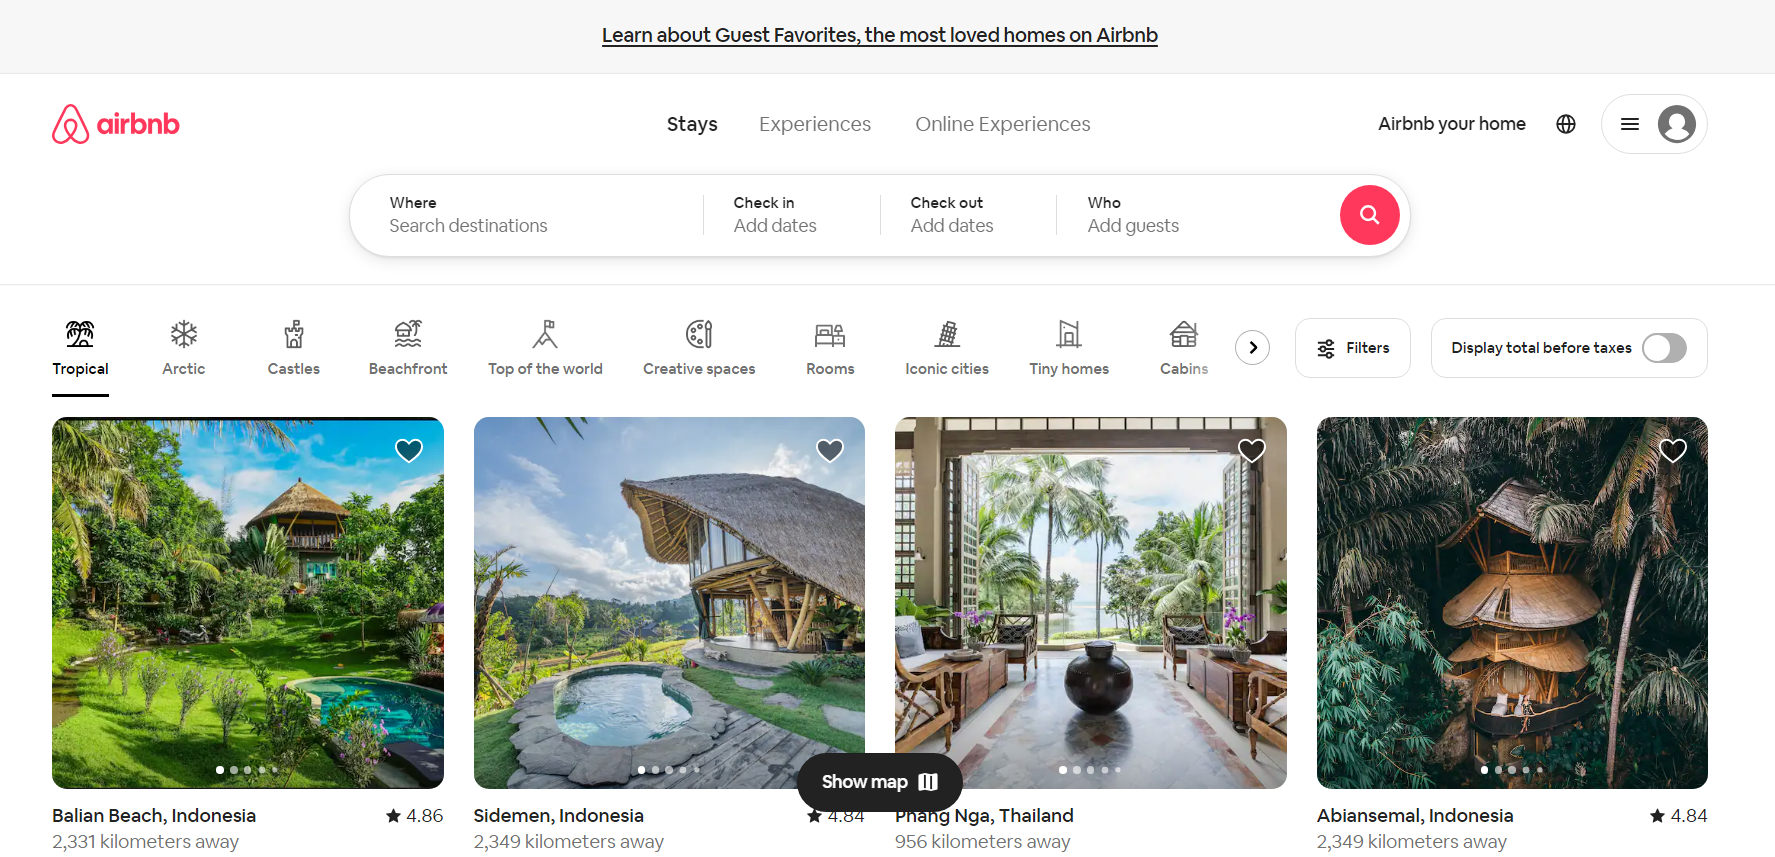
\includegraphics[width=1\textwidth]{Images/RelatedSystems/AirbnbDesktop.png}
    \caption{Giao diện Airbnb trên website}
\end{figure}
\begin{figure}[H]
    \centering
    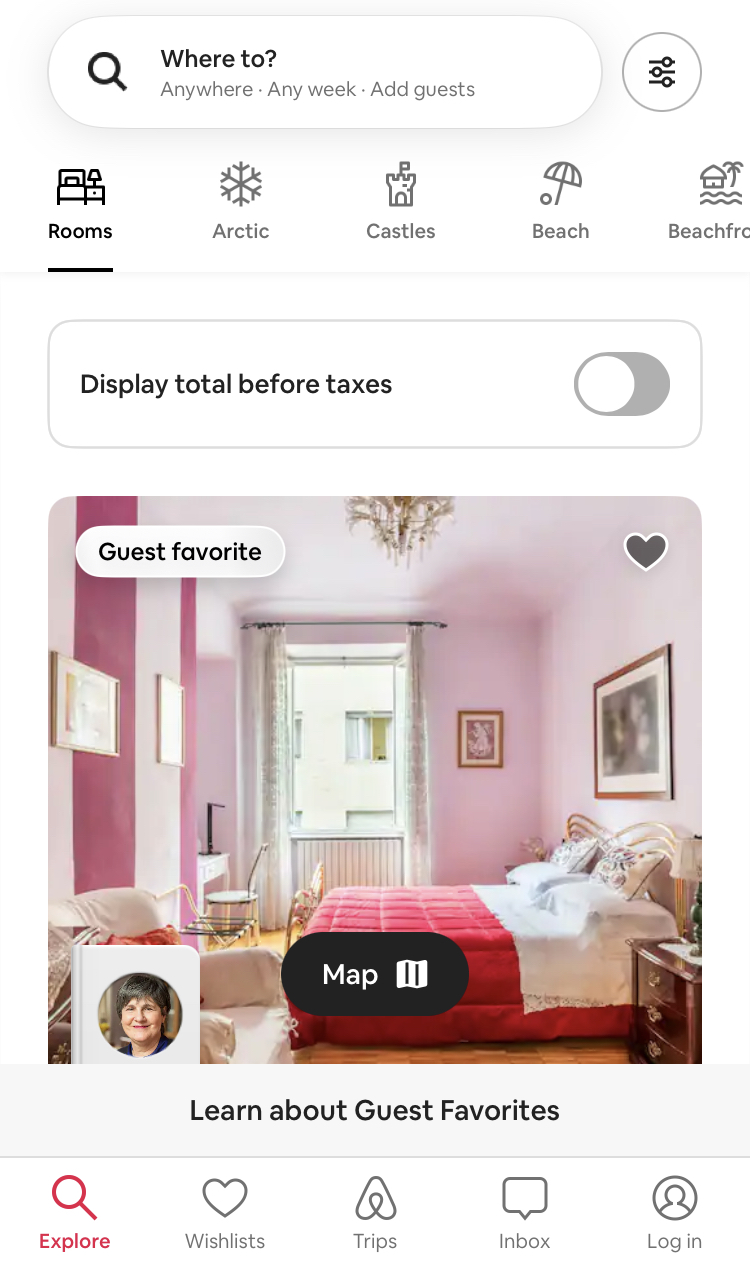
\includegraphics[width=0.5\textwidth]{Images/RelatedSystems/AirbnbMobile.PNG}
    \caption{Giao diện Airbnb trên thiết bị di động}
\end{figure}
\subsubsection{Các tính năng chính}
Airbnb là một nền tảng trực tuyến kết nối người cho thuê nhà/phòng với người tìm nơi ở. Airbnb cung cấp nhiều tính năng khác nhau, bao gồm:
\begin{itemize}
    \item \textbf{Tìm kiếm}
    \begin{itemize}
        \item \textit{Tìm kiếm theo vị trí:} Khách hàng có thể tìm kiếm chỗ ở theo vị trí, chẳng hạn như thành phố, quận, khu phố,...
        \item \textit{Tìm kiếm theo giá cả:} Khách hàng có thể tìm kiếm chỗ ở theo mức giá, chẳng hạn như giá rẻ, giá trung bình, giá cao,...
        \item \textit{Tìm kiếm theo loại chỗ ở:} Khách hàng có thể tìm kiếm chỗ ở theo loại, chẳng hạn như nhà riêng, căn hộ, phòng khách sạn,...
        \item \textit{Tìm kiếm theo tiện nghi:} Khách hàng có thể tìm kiếm chỗ ở có các tiện nghi mong muốn, chẳng hạn như hồ bơi, phòng tập thể dục,...
    \end{itemize}
    \item \textbf{Đặt phòng}
    \begin{itemize}
        \item \textit{Đặt phòng trực tuyến:} Khách hàng có thể đặt phòng chỗ ở trên Airbnb một cách dễ dàng và nhanh chóng.
        \item \textit{Thanh toán linh hoạt:} Airbnb cung cấp nhiều phương thức thanh toán khác nhau để khách hàng lựa chọn, chẳng hạn như thẻ tín dụng, thẻ ghi nợ, PayPal,...
        \item \textit{Hoàn tiền linh hoạt:} Airbnb có chính sách hoàn tiền linh hoạt, giúp khách hàng an tâm khi đặt phòng.
    \end{itemize}
    \item \textbf{Thông tin chỗ ở}
    \begin{itemize}
        \item \textit{Ảnh và video:} Airbnb cung cấp ảnh và video chi tiết về từng chỗ ở, giúp khách hàng có thể hình dung được chỗ ở trước khi đặt phòng.
        \item \textit{Mô tả:} Airbnb cung cấp mô tả chi tiết về từng chỗ ở, bao gồm các thông tin như diện tích, số phòng ngủ, số phòng tắm, tiện nghi,...
        \item \textit{Đánh giá:} Airbnb cung cấp đánh giá của khách hàng đã từng ở chỗ ở, giúp khách hàng có thể đánh giá chất lượng của chỗ ở.
    \end{itemize}
    \item \textbf{Tương tác}
    \begin{itemize}
        \item \textit{Gửi tin nhắn}: Khách hàng có thể gửi tin nhắn cho chủ nhà để trao đổi thông tin, đặt câu hỏi...
        \item \textit{Trao đổi qua Airbnb:} Khách hàng có thể trao đổi với chủ nhà thông qua các công cụ của Airbnb, chẳng hạn như cuộc gọi video, cuộc gọi thoại...
    \end{itemize}
    \item \textbf{Hỗ trợ}
    \begin{itemize}
        \item \textit{Hỗ trợ 24/7:} Airbnb cung cấp dịch vụ hỗ trợ khách hàng 24/7, giúp khách hàng có thể giải quyết các vấn đề trong quá trình sử dụng dịch vụ.
        \item \textit{Trung tâm trợ giúp:} Airbnb cung cấp trung tâm trợ giúp với nhiều tài nguyên hữu ích, giúp khách hàng có thể tự giải quyết các vấn đề.
    \end{itemize}
    \item \textbf{Tính năng bổ sung}
    \begin{itemize}
        \item \textit{Trải nghiệm:} Airbnb cung cấp các trải nghiệm độc đáo, do người dân địa phương tổ chức. Trải nghiệm này giúp khách hàng có thể khám phá văn hóa và con người của địa phương.
        \item \textit{Airbnb for Work:} Airbnb cung cấp các dịch vụ dành riêng cho doanh nghiệp, chẳng hạn như quản lý chuyến công tác, thanh toán theo nhóm,...
    \end{itemize}
\end{itemize}
Ngoài các tính năng trên, Airbnb còn cung cấp một số tính năng khác, chẳng hạn như:
\begin{itemize}
    \item \textbf{Bảo hiểm:} Airbnb cung cấp bảo hiểm cho khách hàng, giúp khách hàng được bảo vệ trong trường hợp xảy ra sự cố.
    \item \textbf{AirCover:} Airbnb cung cấp tính năng AirCover cho khách hàng, giúp khách hàng được bảo vệ trong trường hợp chỗ ở không như mong đợi.
    \item \textbf{Tính toán thuế:} Airbnb cung cấp tính năng tính toán thuế cho khách hàng, giúp khách hàng có thể dễ dàng tính toán thuế khi đặt phòng.
\end{itemize}
\subsubsection{Phân tích SWOT}
\begin{tcbraster}[raster columns=2, boxrule=0mm, arc=0mm]
\begin{tcolorbox}[equal height group=A, size=fbox, colback=swotS!60, colframe=swotS!80!black, title=\textsc{strengths}]
\begin{itemize}
\item Airbnb là công ty tiên phong trong lĩnh vực kinh tế chia sẻ, tạo ra một mô hình mới cho ngành dịch vụ lưu trú.
\item Airbnb cung cấp chỗ ở với mức giá cạnh tranh hơn so với khách sạn truyền thống, phù hợp với nhu cầu của nhiều đối tượng khách hàng.
\item Tốc độ tăng trưởng ấn tượng trong những năm gần đây, với hàng triệu lượt đặt phòng mỗi đêm trên toàn thế giới.
\item Airbnb có lượng dữ liệu khách hàng khổng lồ, giúp công ty hiểu rõ nhu cầu và hành vi của khách hàng, từ đó cải thiện chất lượng dịch vụ.
\end{itemize}
\end{tcolorbox}
\begin{tcolorbox}[equal height group=A, size=fbox, colback=swotW!60, colframe=swotW!80!black, title=\textsc{weaknesses}]
\begin{itemize}
\item Airbnb không trực tiếp quản lý chất lượng dịch vụ của các chủ nhà, dẫn đến một số trường hợp khách hàng gặp phải chất lượng dịch vụ không như mong đợi.
\item Một số vụ bê bối liên quan đến Airbnb, đã gây ảnh hưởng xấu đến hình ảnh thương hiệu của công ty.
\item Ở một số quốc gia, tính pháp lý của Airbnb vẫn chưa được rõ ràng, dẫn đến những rủi ro cho công ty.
\item Airbnb đang phải đối mặt với sự cạnh tranh ngày càng tăng từ các đối thủ như Booking.com, Expedia,...
\end{itemize}
\end{tcolorbox}
\begin{tcolorbox}[equal height group=B, size=fbox, colback=swotO!60, colframe=swotO!80!black, title=\textsc{opportunities}]
\begin{itemize}
\item Ngành du lịch đang có xu hướng tăng trưởng mạnh mẽ, tạo ra nhiều cơ hội cho Airbnb.
\item Sự phát triển của công nghệ, chẳng hạn như trí tuệ nhân tạo, sẽ giúp Airbnb cải thiện chất lượng dịch vụ và trải nghiệm của khách hàng.
\item Airbnb có thể mở rộng sang các thị trường mới, chẳng hạn như các thị trường đang phát triển, để tiếp cận nhiều khách hàng hơn.
item Airbnb có thể phát triển các sản phẩm và dịch vụ mới, chẳng hạn như dịch vụ cho thuê xe, dịch vụ ăn uống,... để đáp ứng nhu cầu ngày càng đa dạng của khách hàng.
\end{itemize}
\end{tcolorbox}
\begin{tcolorbox}[equal height group=B, size=fbox, colback=swotT!60, colframe=swotT!80!black, title=\textsc{threats}]
\begin{itemize}
\item Xu hướng du lịch có thể thay đổi theo thời gian, dẫn đến những thách thức cho Airbnb.
\item Sự phát triển của các công nghệ mới, chẳng hạn như thực tế ảo, có thể thay đổi cách thức du lịch của mọi người, dẫn đến những thách thức cho Airbnb.
\item Các quy định và thuế mới có thể ảnh hưởng đến hoạt động kinh doanh của Airbnb.
\item Kinh tế suy thoái có thể dẫn đến giảm nhu cầu du lịch, từ đó ảnh hưởng đến doanh thu của Airbnb.
\end{itemize}
\end{tcolorbox}
\captionof{table}{Phân tích SWOT cho Airbnb}
\end{tcbraster}
\subsubsection{Nhận xét}
\hspace*{1cm}Airbnb, với định dạng đặt phòng trực tuyến độc đáo, đã làm thay đổi bối cảnh của ngành du lịch và góp phần tạo ra một mô hình động mới cho việc tương tác với môi trường địa phương. Nền tảng này không chỉ mang lại sự linh hoạt và đa dạng trong việc lựa chọn chỗ ở, từ những căn hộ hiện đại đến những ngôi nhà truyền thống, mà còn mở ra một cửa sổ rộng lớn để du khách tương tác với văn hóa địa phương một cách chân thực.\\
\hspace*{1cm}Trải nghiệm của du khách trên Airbnb không chỉ là việc tìm kiếm nơi lưu trú, mà còn là việc kết nối với cộng đồng địa phương thông qua việc ở chung với các chủ nhà địa phương. Sự ấm cúng và thuận tiện được cung cấp bởi các chỗ ở này không chỉ giúp tạo ra không gian thoải mái cho du khách mà còn đóng góp vào sự đa dạng và sâu sắc của trải nghiệm du lịch.\\ \hspace*{1cm}Tuy nhiên, trong bối cảnh lớn và đa dạng như vậy, việc quản lý chất lượng và an toàn trở nên quan trọng. Các vấn đề như đánh giá chủ nhà, phản hồi từ cộng đồng, và các biện pháp an ninh cần được xem xét một cách cẩn thận để đảm bảo rằng môi trường Airbnb duy trì một tiêu chuẩn cao về chất lượng dịch vụ và an toàn cho mọi du khách.